\documentclass[aspectratio=169,xcolor=pdftex,dvipsnames,table]{beamer}\usepackage[]{graphicx}\usepackage[]{xcolor}
% maxwidth is the original width if it is less than linewidth
% otherwise use linewidth (to make sure the graphics do not exceed the margin)
\makeatletter
\def\maxwidth{ %
  \ifdim\Gin@nat@width>\linewidth
    \linewidth
  \else
    \Gin@nat@width
  \fi
}
\makeatother

\definecolor{fgcolor}{rgb}{0.345, 0.345, 0.345}
\newcommand{\hlnum}[1]{\textcolor[rgb]{0.686,0.059,0.569}{#1}}%
\newcommand{\hlstr}[1]{\textcolor[rgb]{0.192,0.494,0.8}{#1}}%
\newcommand{\hlcom}[1]{\textcolor[rgb]{0.678,0.584,0.686}{\textit{#1}}}%
\newcommand{\hlopt}[1]{\textcolor[rgb]{0,0,0}{#1}}%
\newcommand{\hlstd}[1]{\textcolor[rgb]{0.345,0.345,0.345}{#1}}%
\newcommand{\hlkwa}[1]{\textcolor[rgb]{0.161,0.373,0.58}{\textbf{#1}}}%
\newcommand{\hlkwb}[1]{\textcolor[rgb]{0.69,0.353,0.396}{#1}}%
\newcommand{\hlkwc}[1]{\textcolor[rgb]{0.333,0.667,0.333}{#1}}%
\newcommand{\hlkwd}[1]{\textcolor[rgb]{0.737,0.353,0.396}{\textbf{#1}}}%
\let\hlipl\hlkwb

\usepackage{framed}
\makeatletter
\newenvironment{kframe}{%
 \def\at@end@of@kframe{}%
 \ifinner\ifhmode%
  \def\at@end@of@kframe{\end{minipage}}%
  \begin{minipage}{\columnwidth}%
 \fi\fi%
 \def\FrameCommand##1{\hskip\@totalleftmargin \hskip-\fboxsep
 \colorbox{shadecolor}{##1}\hskip-\fboxsep
     % There is no \\@totalrightmargin, so:
     \hskip-\linewidth \hskip-\@totalleftmargin \hskip\columnwidth}%
 \MakeFramed {\advance\hsize-\width
   \@totalleftmargin\z@ \linewidth\hsize
   \@setminipage}}%
 {\par\unskip\endMakeFramed%
 \at@end@of@kframe}
\makeatother

\definecolor{shadecolor}{rgb}{.97, .97, .97}
\definecolor{messagecolor}{rgb}{0, 0, 0}
\definecolor{warningcolor}{rgb}{1, 0, 1}
\definecolor{errorcolor}{rgb}{1, 0, 0}
\newenvironment{knitrout}{}{} % an empty environment to be redefined in TeX

\usepackage{alltt}
% \documentclass[notes,aspectratio=169,xcolor=pdftex,dvipsnames,table]{beamer}

%\setbeameroption{show notes}

\usepackage{bm,graphicx,amsmath,tikz} %fancybox,
\usepackage{color}%,textpos}
\usepackage[round]{natbib}
\usepackage[normalem]{ulem}
\usepackage{hyperref}
\usepackage{lastpage}
\usepackage{array}
\usepackage{color}
\usepackage{framed}
\usepackage{mathtools}

% Define Western colours
\definecolor{western}{rgb}{.306,.152,.524}
\definecolor{westerngray}{rgb}{.512,.508,.524}

%% Define BEAMER colours
\setbeamercolor{frametitle}{bg=western,fg=white}
\setbeamercolor{framesubtitle}{bg=western,fg=black}
\setbeamercolor{title}{fg=white,bg=western}
\setbeamercolor{author}{fg=white,bg=western}
\setbeamercolor{institute}{fg=white,bg=western}
\setbeamercolor{date}{fg=white,bg=western}

%% Set BEAMER fonts
\setbeamerfont{title}{shape=\bf}
\setbeamerfont{frametitle}{shape=\sc,size=\Large}
\setbeamerfont{framesubtitle}{shape=\sc,size=\Large}
\setbeamerfont{footline}{shape=\sc}

%% Define BEAMER toc
\setbeamercolor{section in toc}{fg=western}
\setbeamercolor{subsection in toc}{fg=westerngray}
\setbeamertemplate{sections/subsections in toc}[ball]

%% Define BEAMER background
\setbeamercolor{background canvas}{bg=white}

%% Define BEAMER footer
\setbeamertemplate{navigation symbols}{}
\setbeamercolor{footline}{fg=white,bg=western}
\setbeamertemplate{footline}{%
  \begin{beamercolorbox}[wd=\paperwidth]{footline}
    \vskip5pt

    \hspace{.1in}
    \raisebox{.05in}{
      \scriptsize{\bf \insertshorttitle }
    }
    \hfill
    \raisebox{.05in}{
      \scriptsize{\bf \insertframenumber/\pageref{LastPage}}
    }
    \hspace{5pt}

    \vskip5pt
  \end{beamercolorbox}
}

%% Define BLOCK environment
\setbeamercolor{block title}{fg=western}
\setbeamerfont{block title}{series=\bfseries}

%% Define ENUMERATE and ITEMIZE environements
\setbeamertemplate{itemize item}[ball]
\setbeamertemplate{enumerate item}[ball]
\setbeamercolor{item projected}{bg=western}

%% Define BEAMER toc
\setbeamercolor{sections/subsections in toc}{fg=blue!75}
\setbeamertemplate{sections/subsections in toc}[ball]

%% Define SECTION openings
\AtBeginSection[]{
}

\title[SS2857 -- Lecture 3]{SS2857 Probability and Statistics 1\\
  Fall 2024\\
  \vspace{.2in}
  Lecture 3}
  
\date{Revised 18/09/24}



\IfFileExists{upquote.sty}{\usepackage{upquote}}{}
\begin{document}

{
\setbeamertemplate{footline}{}
\setbeamercolor{background canvas}{bg=western}

\begin{frame}
  \maketitle
\end{frame}
}


\begin{frame}
  \begin{center}
    \Large{\textbf{2.3 Counting Techniques}}

    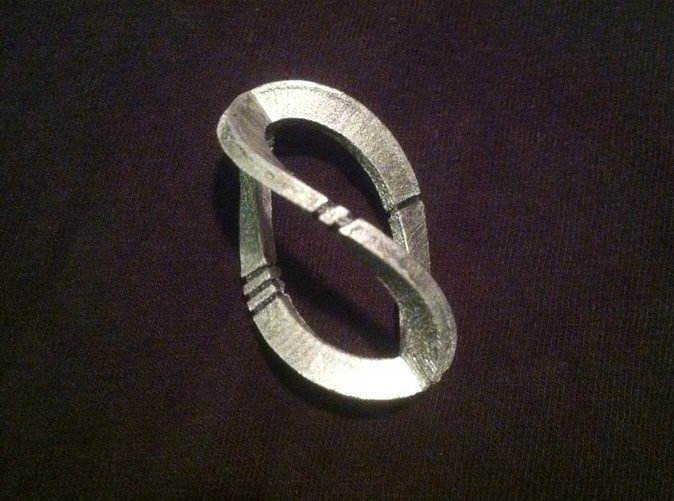
\includegraphics[height=.6\textheight]{three_sided_die}
  \end{center}
\end{frame}

\begin{frame}{Equally Likely Outcomes}

  If all outcomes in the sample space are equally likely, the probability of any simple event is $1/N$, then the probability of any event is
  \[
    P(A)=\frac{n(A)}{A}.
  \]
  
\end{frame}

\begin{frame}{Example 3.1}
  Suppose that you roll a (fair) three-sided die\footnote{https://www.cnet.com/news/this-3d-printed-3-sided-die-is-a-work-of-modern-art/} three times.

  \medskip

  \begin{enumerate}[a)]
  \item What is the probability that you never roll a three?
  \item What is the probability that the sum is greater than 4?
  \item What is the probability that the number rolled is less than three every time or the sum \textcolor{red}{greater than} 4?
  \end{enumerate}
  
\end{frame}


\begin{frame}{Permutations and Combinations}
  \begin{block}{Permutations}
    Count the number of ways to draw $k$ of $n$ distinct objects \textit{without replacement} when order matters. I.e., two outcomes are considered the same if they contain the same elements \textit{in the same order}.
    \[
      \prescript{}{n}P_k=n(n-1)(n-2)\cdots(n-k+1)=\frac{n!}{(n-k)!}
    \]
  \end{block}

  \vspace{-.2in}
  
  \begin{block}{Combinations}
    Count the number of ways to draw $k$ of $n$ distinct objects \textit{without replacement} when order \textcolor{red}{does not} matter. I.e., two outcomes are considered the same if they contain the same elements \textit{in any order}.
    \[
      \prescript{}{n}C_k={n \choose k} =\frac{n!}{k!(n-k)!}=\frac{P_{k,n}}{k!}
    \]
  \end{block}
  
\end{frame}

\begin{frame}{Example 3.2}
  Identify whether each of the following is a permutation or a combination. What are the values?

  \medskip

  The number of:
  \begin{enumerate}[a)]
  \item hands of 5 cards that can be dealt from a standard deck of 52 unique cards.
  \item ways for four people to line up.
  \item selections on the Lotto 6/49.
  \item teams of 10 students that are possible in a class of 150.
  \item create 2 lines of 10 from a class of 30 students.
  \end{enumerate}
\end{frame}

\begin{frame}{Example 3.3}
  A standard deck of cards contains 13 cards (A,2,3,$\ldots$,10,J,Q,K) in each of 4 suits (Clubs, Diamonds, Hearts, Spades).

  \begin{enumerate}[a)]
  \item What is the probability that you are dealt a royal flush (\textcolor{red}{10, J, Q, K, A}) in the same suit)?
    
  \item What is the probability that you are dealt a royal flush in order?
  
  \item c) What is the probability that you are dealt a pair (two cards of one face value and three cards of other non-matching face values)?
  
  \item What is the probability of getting a full-house (two cards of one face value and three of another?
  \end{enumerate}
  
\end{frame}

\begin{frame}{Formatting Solutions}
  \begin{enumerate}
  \item Define your events (or any other variables)\\
    Write:
    \begin{quote}
      Let $C$ be the event that the sky is blue. Then $P(C)=\cdots$
    \end{quote}
    Not:
    \begin{quote}
      \[
        P(\mbox{the sky is blue})=\cdots
      \]
    \end{quote}
  \item Keep extra (5 or 6) significant figures in your work to ensure that you don't commit rounding errors:
    \[
      P(C)=\frac{3744}{2,598,960}=.001441.
    \]
    
  \item Finish with a clear conclusion so we don't need to guess which number is your final answer. Round your final answer to 2 or 3 significant figures.
    \begin{quote}
      The probability of the event is $.0014$. 
    \end{quote}
  \end{enumerate}
  
\end{frame}

\begin{frame}
  \begin{center}
    \Large{\textbf{Questions?}}
  \end{center}
\end{frame}

\begin{frame}{Exercise 3.1}

Consider Example 3.3. Show the following:

\begin{enumerate}[a)]
\item The probability of being dealt a flush (all 5 cards from one suit) is .00198.
\item The probability of being dealt two pairs (a pair of one value, a pair of another, and one other card) is .0475.
\item The probability of being dealt three of a kind (three of one value, one of another value, and one of yet another) is .0211.
\end{enumerate}
\end{frame}


\end{document}
